\documentclass[a4paper, 14pt, russian]{article}
\usepackage[a4paper]{geometry}
\usepackage{mathtext}
\usepackage{lipsum}
\usepackage{extsizes}
\usepackage{cmap}
\usepackage{caption}
\usepackage[T2A]{fontenc}
\usepackage[utf8]{inputenc}
\usepackage[russian]{babel}
\usepackage{physics}
\usepackage{hyperref}
\usepackage{indentfirst}
\usepackage{fancyhdr}
\usepackage{enumerate}
\usepackage{amssymb, amsmath}
\usepackage{tikz}
\usepackage{pgfplots}
\usepackage{mdwlist}
\usepackage{apacite}
\geometry{left=3cm,right=1.5cm,top=2cm,bottom=2cm}
\usepackage[unicode]{hyperref}  %создаёт гиперссылки на список литературы в pdf-файле
\linespread{1.3}                % полтора интервала. Если 1.6, то два интервала
\begin{document}
\begin{titlepage}
\begin{center}
\textbf{МИНИСТЕРСТВО НАУКИ И ВЫСШЕГО ОБРАЗОВАНИЯ РОССИЙСКОЙ ФЕДЕРАЦИИ}

\vspace{0.3cm}

\textbf{Национальный исследовательский университет}

\textbf{Высшая школа экономики}

\vspace{0.3cm}

Факультет информатики, математики и компьютерных наук
\end{center}


\begin{center}
\Large{\bf{Вероятностная модель транспортных потоков на автомагистрали}}
\end{center}

\vspace{0.3cm}

\begin{flushright}
Курсовая работа

студента 1 курса магистратуры

специальности ''Интеллектуальный анализ данных'',

Шилова Андрея Сергеевича

% \vspace{6\mytextsize}
\vspace{0.5 cm}
\underline{Научный руководитель:}

Кандидат физико-математических наук

Федоткин Андрей Михайлович

\end{flushright}

\vspace{9cm}

\begin{center}
Нижний Новгород

2020 г.
\end{center}

\end{titlepage}

\tableofcontents                % Автоматическое создание оглавления по названиям разделов, подразделов и т.п.

\newpage

\section{Введение}

С развитием транспортной индустрии в последние полвека остро возникла проблема чрезмерной загруженности транспортных потоков как в городах, так и на автомагистралях. Для решения этой проблемы по всему миру общественностью принимается множество мер:
\begin{itemize}
\item Депопуляризации личного транспорта. 23 сентября каждого года по всему миру проводится всемирный ''день без автомобиля'' (\url{https://opennov.ru/news/society/2019-09-22/20939})
\item Создание программ развития общественного транспорта (\url{https://www.mintrans.ru/images/content/gos-programma-rasv-tran-sist.pdf}). Известно, что каждый автобус или вагон метро средней заполненности приблизительно в 20 раз более эффективен с точки зрения загрузки транспортного потока, чем аналогичное по вместительности пассажиров количество личных автомобилей. Развивая инфраструктуру общественного транспорта, возможно значительно разгрузить дорожные пути.
\item Оптимизация системы дорожного движения. Для обеспечения эффективного дорожного движения необходимо отрегулировать систему управления транспортными потоками таким образом, чтобы создать максимально однородное по скорости и координатам распределение автомашин. В отличие от предыдущих двух, эта мера действует как для городских, так и для магистральных транспортных путей.
\end{itemize}

Целью данной работы является исследование существующих вероятностных моделей дорожного движения на автомагистрали. Имея математическую модель, возможно воссоздать более точную картину проблем, связанных с дорожным движением на автомагистралях, и путей их решения.
\section{Описание вероятностной модели}

Мы будем рассматривать одномерный поток автомобилей на автомагистрали. Введем две  случайных величины:

\begin{itemize}
\item $\eta(t), t > 0$ - число машин, пересекших некоторую случайную линию с координатой \textit{x} за промежуток времени (0, t). При этом $\eta(0) = 0$.
\item $\nu(x), x > 0$ - число машин, располагающихся на участке дороги (0,x) в момент времени t. При этом $\nu(0) = 0$.
\end{itemize}

Предположим, что на дороге существует два типа автомобилей: ''быстрые'' и ''медленные''. Наблюдения показывают, что движение на автомагистрали при плохих погодных условиях происходит по следующему принципу: из-за сложности совершения обгона в таких условиях образуются колонны (пачки) ''быстрых'' автомобилей, возглавляемые "медленным" автомобилем. Колонна пополняется, когда ее догоняет очередной "быстрый" автомобиль, и уменьшается, когда происходит обгон головного "медленного" автомобиля. Пачки автомобилей при этом считаются независимыми.

\subsection{Идеальные условия}
При хороших условиях (прямой участок дороги с хорошей видимостью и сухом дорожном покрытии) движение автомобилей по автомагистрали является совокупностью независимых движений каждого автомобиля. С точки зрения дорожного движения это связано с тем, что маневр обгона не представляет сложности, и задержка при опережении медленного автомобиля быстрым минимальна. В таком случае распределение являетcя пуассоновским.
\textit{**Место для доказательства; ссылка 136 в диссертации**}

\subsection{Плохие погодные условия}
При плохих погодных условиях предположение о независимости движений автомобилей, движущихся с разной скоростью, не выполняется. В данном случае необходима более сложная модель.

Введем следующие обозначения:
\begin{itemize}

\item $\eta_0(t)$ - случайное число быстрых автомобилей, поступающих в колонну. Исходя из предыдущего раздела,
$P(\{\eta_0(t) = k\}) = \frac{\lambda_0^k}{k!}e^{- \lambda_0}$,
где $\lambda_0$ - параметр распределения Пуассона, интерпретируемый как интенсивность поступления ''быстрых'' машин в пачку.

\item $\varkappa_0(t)$ - случайная величина, обозначающая количество автомобилей всех типов в пачке, принимающее значения {1 ... N}.

\item $\xi_0(t, \Delta t)$ - случайная величина, обозначающая число быстрых автомобилей, совершающих обгон в промежуток времени $(t, t + \Delta t)$
\end{itemize}

Можно получить следующие равенства:

\begin{enumerate} 
\item Так как движение быстрых машин на автомагистрали можно считать равномерным, они поступают в пачку по линейному от времени закону. При малых $\Delta t$ можно записать:

$P(\eta_0(t+ \Delta t) - \eta_0(t) = 0) = 1 - \lambda_0 \Delta t + o(\Delta t)$

$P(\eta_0(t+ \Delta t) - \eta_0(t) = 1) = \lambda_0 \Delta t - o(\Delta t)$

\item Предположим, что движение достаточно разреженное, чтобы процессы внутри каждой пачки не оказывали влияния на количество поступающие в нее машины. Тогда $\forall \ t_2 > t_1 \ P(\{\eta_0(t_2) - \eta_0(t_1) = k\})$ зависит только от \textit{k} и разности $t_2 - t_1$, и следовательно $P(\{\eta_0(t_2) - \eta_0(t_1) = k\}) = P({\eta_0(t_2 - t_1) = k}) \ \forall \ k$.

% \end{enumerate} 
\suspend{enumerate}
Пользуясь (1) и условием $\sum_{k = 0}^{\infty}P(\{\eta_0(t+\Delta t) - \eta_0(t) = k\}) = 1$ (формула полной вероятности), можно получить, что $P(\{\eta_0(t+\Delta t) - \eta_0(t) \geq 2 \}) = o(\Delta t)$ - вероятность того, что при малом $\Delta t$ пачку догонит более чем одна машина, мала. Это согласуется с правилами дорожного движения. Такое соображение позволяет не рассматривать события, связанные с изменением величин $\eta_0, \xi_0, \varkappa_0$ более, чем на единицу, так как их вероятность мала.


\resume{enumerate}
% \begin{enumerate}
\item Рассмотрим условные вероятности событий:

$P(\{\xi_0(t, \Delta t) = 0\} | \{ \varkappa_0(t, \Delta t) = 1, \eta_0(t, \Delta t) = 0\}) = 1$

Физический смысл этого равенства состоит в том, что автомобиль не может совершить обгон, будучи единственным в пачке.

$P(\{\xi_0(t, \Delta t) = 0\} | \{ \varkappa_0(t, \Delta t) = 1, \eta_0(t, \Delta t) = 1\}) = 1 - O(\Delta t)$

Это равенство означает, что машина, только что присоединившаяся к колонне, не будет совершать обгон с линейно убывающей со временем вероятностью.

\suspend{enumerate}
Пользуясь таким линейным приближением, запишем:
\resume{enumerate}

\item $P(\{\xi_0(t, \Delta t) = 0\} | \{\varkappa_0(t, \Delta t) = 2, \eta_0(t, \Delta t) = 0\}) =  1 - \mu_{1, 0} \Delta t + o(\Delta t)$

$P(\{\xi_0(t, \Delta t) = 1\} | \{\varkappa_0(t, \Delta t) = 2, \eta_0(t, \Delta t) = 0\}) =  \mu_{1, 0} \Delta t - o(\Delta t)$, 

где параметр $\mu_{1,0}$ задает интенсивность обгона медленных машин быстрыми в случае, когда пачка состоит из двух машин. Его значение связано с погодными условиями.

\item $P(\{\xi_0(t, \Delta t) = 0\} | \{\varkappa_0(t, \Delta t) = k, \eta_0(t, \Delta t) = 0\}) =  1 - \mu_{2, 0} \Delta t + o(\Delta t)$

$P(\{\xi_0(t, \Delta t) = 1\} | \{\varkappa_0(t, \Delta t) = k, \eta_0(t, \Delta t) = 0\}) =  \mu_{2, 0} \Delta t - o(\Delta t)$ 

$\forall k = 3, 4, ... N -1$, где параметр $\mu_{2,0}$ задает интенсивность обгона медленных машин быстрыми в случае, когда пачка состоит из более чем двух машин. Различие между параметрами $\mu_{1,0}$ и $\mu_{2,0}$ объясняется психологическим различием оценок сложности маневра обгона с точки зрения водителя быстрого автомобиля в зависимости от величины транспортной пачки.

\item Наложим также ограничение на размер пачки: пусть $\exists$ N - такое число машин, что как только N+1 - ая машина догоняет пачку, мгновенно происходит обгон головного медленного автомобиля одним из быстрых. Тогда:

$P(\{\xi_0(t, \Delta t) = 0\} | \{\varkappa_0(t, \Delta t) = N, \eta_0(t, \Delta t) = 0\}) = 1 -  \mu_{2, 0} \Delta t + o(\Delta t)$ 

$P(\{\xi_0(t, \Delta t) = 1\} | \{\varkappa_0(t, \Delta t) = N, \eta_0(t, \Delta t) = 0\}) = \mu_{2, 0} \Delta t - o(\Delta t)$ 

 $P(\{\xi_0(t, \Delta t) = 1\} | \{\varkappa_0(t, \Delta t) = N, \eta_0(t, \Delta t) = 1\}) = 1$

\end{enumerate} 

\subsection{Переход к дифференциальным уравнениям}

Пользуясь полученными выше выражениями, получим уравнение на размер пачки. Обозначим $Q(t, k) = P(\{\varkappa_0(t) = k\})$.

Условие, что количество автомобилей сохраняется:

$\varkappa_0(t + \Delta t, k) = \varkappa_0(t, k) + \mu_o(t) - \xi_0(t)$

Рассматривая линейное приближение, в котором не малы только вероятности событий, включающих действие лишь одного автомобиля (увеличение или уменьшение пачки на один автомобиль), можно записать:

$P(\{\varkappa_0(t + \Delta t) = k\}) = P(\{\varkappa_0(t) = k\} | \{\xi_0(t) = 0, \eta_0(t) = 0\}) + P(\{\varkappa_0(t) = k-1\} | \{\xi_0(t) = 0, \eta_0(t) = 1\}) + 
P(\{\varkappa_0(t) = k+1\} | \{\xi_0(t) = 1, \eta_0(t) = 0\}) + o(\Delta t)$,

или

$Q(t + \Delta t, k) = (1 - \lambda_0 \Delta t - \mu_{2,0} \Delta t ) Q(t, k) + (\mu_{2,0} \Delta t) Q(t, k+1) + \lambda_0 Q(t, k-1) + o(\Delta t)$

$\Delta t \rightarrow 0\Rightarrow $

$\frac{dQ(t, k)}{dt} = -(\lambda_0 + \mu_{2,0}) Q(t, k) + \mu_{2,0} Q(t, k + 1) + 
\lambda_0 Q(t, k-1)$, \textit{k} = 3, 4 ... N-1

Аналогично:

$\frac{dQ(t, 1)}{dt} = -\lambda_0 Q(t, 1) + \mu_{1,0} Q(t, 2)$

$\frac{dQ(t, 2)}{dt} = -(\lambda_0 + \mu_{1,0}) Q(t, 2) + \mu_{2,0} Q(t, 3) + 
\lambda_0 Q(t, 1)$

$\frac{dQ(t, N)}{dt} = - \mu_{2,0} Q(t, N) + \lambda_0 Q(t, N - 1)$

Начальные условия могут быть заданы в виде:

$Q(0, i) = 1, Q(0, k) = 0 \ \forall k \neq i$ для выбранного $i = 1 ... N$
Полученная  система из N линейных дифференциальных уравнений с заданными начальными условиями описывает динамику движения транспортных пачек на автомагистрали.

\subsection{Решение системы дифференциальных уравнений}
Рассмотрим случай транспортной пачки, состоящей из двух машин.

\textit{**Рассмотрим позднее**}

\subsection{Результаты численного моделирования}

С помощью пакета \textit{scipy} было проведено численное решение для различных параметров $\lambda_0, \ \mu_{1,0}, \ \mu_{2,0}, \ N$ и начальных условий. Результаты приведены на рис. 1, 2:

\begin{figure}[!ht]
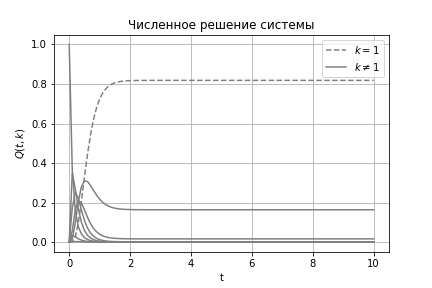
\includegraphics[width=0.8\textwidth]{pictures/1.jpg}
\caption{Численное решение для параметров $\lambda_0 = 1, \mu_{1,0} = 5, \mu_{2,0} = 10, N = 10, Q(0, 4) = 1$ - распад транспортной пачки}
\centering
\end{figure}

\begin{figure}[!ht]
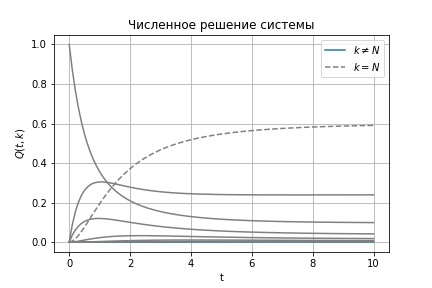
\includegraphics[width=0.8\textwidth]{pictures/2.jpg}
\caption{Численное решение для параметров $\lambda_0 = 1, \mu_{1,0} = 0.25, \mu_{2,0} = 0.4, N = 10, Q(0, 4) = 1$ - образование затора}
\centering
\end{figure}

Из этих графиков возможно сделать следующий вывод: в зависимости от величин параметров $\lambda_0, \mu_{1,0}, \mu_{2,0}$ при $t \rightarrow \infty$ могут устанавливаться различные стационарные распределения, причем при условии $\lambda_0 \gg \mu_{1,0}, \mu_{2,0}$ (пуассоновский приток автомобилей в пачку велик по сравнению с интенсивностями обгона) с наибольшей вероятностью образуется затор, в то время как при обратном условии $\lambda_0 \ll \mu_{1,0}, \mu_{2,0}$ все быстрые машины обгоняют головной медленный автомобиль. Этот вывод верен независимо от значений N и начальных условий.
\section{Экспериментальная проверка модели}

\section{Заключение}

\section{Список литературы}
\end{document}